\chapter{Experiments}\label{Experiments chapter}
In this chapter we will through experiments investigate what speedup one might get by using the algorithm for parallelizing optimal control problems with  time dependent DE constraints in temporal direction, introduced in previous chapters. Unlike the parallel performance of gradient and objective function evaluation, the parallel performance of our overall algorithm is difficult to model. The reason for this is that it is difficult to say how many gradient and function evaluations are needed for the optimization algorithms to terminate. We are therefore unable to derive any theoretical expected speedup.
\\
\\
In section \ref{analysis sec} we explained that the best way of measuring performance of a parallel algorithm is to compare its execution time to the sequential execution time of the best sequential algorithm. When solving optimal control problems with DE constraints, the runtime of our solution algorithm will depend on how many times we have to evaluate the objective function and its gradient, since these evaluations require either the solution of the state equation or the state and adjoint equations. We know from theory in section \ref{analysis sec} and verification in section \ref{ver S sec}, that the speedup of parallel gradient and function evaluation depends linearly on the number of processes we use. An alternative way of measuring parallel performance is therefore to compare the sum of gradient and function evaluations in the sequential and parallel algorithms. Let us give this numbers a name:
\begin{align*}
L_s &= \textit{Number of function and gradient evaluations for sequantial algorithm}\\
L_{p_N} &= \textit{Number of function and gradient evaluations for parallel algorithm using N processes}
\end{align*} 
Using these definitions we define the ideal speedup $\hat{S}$, as the speedup one would expect based on $L_s$ and $L_{p_N}$ and the speedup results we have for function and gradient evaluations:
\begin{align}
\hat S = \frac{NL_s}{L_{p_N}} \label{ideal S}
\end{align}
With $\hat S$, it is possible to say something about the performance of the parallel algorithm without having to time it, or actually run it in parallel. It will also be useful to compare the ideal speedup with the measured speedup, as a way to check if the parallel implementation is implemented efficiently.
\section{Testing Parareal-based preconditioner for example problem}
In this section we will test the parallel framework introduced in chapter \ref{method_chap} on our example problem (\ref{exs_J}-\ref{exs_E}). To be able to do this, we need to define a specific objective function and state equation. The problem we will look at in this section is the following:
\begin{align}
&J(y,v) = \frac{1}{2}\int_0^{100}v(t)^2dt + \frac{1}{2}(y(100)-11.5)^2, \label{speed_j}\\
&\left\{
     \begin{array}{lr}
       	y'(t)=-0.097y(t) + v(t) \quad t\in(0,100)\\
       	y(0)=3.2
     \end{array}
   \right. \label{speed_e}
\end{align}
We motivate the choice of a large end time $T=100$ with the findings of section \ref{consistency_sec}. There we observed that the penalty method ran into trouble when the time steps became too small, because the error in objective function value then hit machine precision. To be able to test the problem for a large number of time steps, we therefore need a large $T$. 
\subsection{Comparing unpreconditioned and preconditioned penalty framework}
In section \ref{pc sec} we introduced the parareal preconditioner, as an approximation to the Hessian. Using this preconditioner in our L-BFGS solver we hope that the number of gradient and function evaluations needed in our algorithm will be smaller than if we do not use it. The experiment is conducted by first solving this problem without decomposing the time interval, and then solving the decomposed problem using $N=2,4,8,16,32,64,128$ decompositions. For all minimizations of the penalized objective function, we used penalty parameter $\mu=10^4$. This means that we will only use one penalty iteration, as we have found this to be the most effective way to solve the decomposed problem for this specific problem. To discretize the equations we have used the Crank-Nicolson scheme with $\Delta t= \frac{T}{1000}=0.1$. For both the penalized and non-penalized problems we use L-BFGS with stop criteria:
\begin{align*}
||\nabla J||_{L^2} <10^{-5}
\end{align*}  
Since the point of this test is to compare the effectiveness of the Parareal-based preconditioner, we solve the decomposed problems with and without it. In table \ref{speed1} we have included the total number of gradient and function evaluations for the two cases as "pc L" and "non-pc L". We also measured the relative $L^2$-norm difference between the exact solution $v_e$ and all the penalized control solutions. The ideal speedup (\ref{ideal S}) is calculated for preconditioned and unpreconditioned solvers.
\\
\\
\begin{table}[h]
\centering
\caption{Comparing unpreconditioned and preconditioned solver for test problem (\ref{speed_j}-\ref{speed_e}) using $N$ decompositions in time. Here $v_e$ denotes the exact control solution, $v_{pc}$ the preconditioned solver control solution and $v$ the unpreconditioned solver solution.}
\label{compare_table}
\begin{tabular}{lrrllrr}
\toprule
{}$N$ &  pc $L_{p_N}$ &  non-pc $L_{p_N}$ &       $||v_e-v_{pc}||$ &  $||v_e-v||$  &  pc $\hat{S}$ &  non-pc $\hat{S}$ \\
\midrule
1   &     19.0 &      19.0 &  0.000174 &    0.000174 &    1.000000 &        1.000000 \\
2   &     21.0 &      21.0 &  0.001093 &    0.001093 &    1.809524 &        1.809524 \\
4   &     45.0 &      45.0 &  0.000640 &    0.000361 &    1.688889 &        1.688889 \\
8   &     61.0 &      69.0 &  0.000667 &    0.001590 &    2.491803 &        2.202899 \\
16  &     61.0 &     241.0 &  0.001608 &    0.000784 &    4.983607 &        1.261411 \\
32  &     73.0 &     343.0 &  0.001909 &    0.002528 &    8.328767 &        1.772595 \\
64  &     67.0 &     737.0 &  0.005273 &    0.004816 &   18.149254 &        1.649932 \\
128 &     67.0 &     907.0 &  0.010892 &    0.018467 &   36.298507 &        2.681367 \\
\bottomrule
\end{tabular}
\end{table}
\\
\\
There are several things of note about the results in table \ref{compare_table}. First off we see that the normed difference in control between exact and parallel solution lies in the range from $10^{-4}$ to $10^{-2}$. Another observation about the norm difference, is that for each $N$, the preconditioned and unpreconditioned solvers seems to produce roughly the same error. 
\\
\\
When we look at the total number of gradient and functional evaluations for the preconditioned and unpreconditioned solvers, we see that there are differences. While it seems to be little to no benefit to use the preconditioner for $N=1,...,8$, it becomes very important for the bigger $N$ values, where number of gradient and functional evaluations seems to explode for the unpreconditioned solver. If one accepts the above solutions as good enough, we see that we for the preconditioned solver get speedup for all decompositions, and that the ideal speedup seems to increase when we increase $N$. We do however see that the ideal speedup for each $N$ is considerably less then optimal for all $N$. Another thing that we notice when looking at the sum of gradient and function evaluations for the preconditioned solver, is that it increases steadily up to $N=8$, and then starts to decline again for higher $N$s. The reason for this is that when we increase the number of decomposed subintervals, we also make the coarse solver in the parareal preconditioner finer. This means that the preconditioner becomes a better approximation of the Hessian, which makes the L-BFGS iteration converge faster.
\subsection{Speedup results for a high number of decompositions}
To properly test the Parareal-based preconditioner, we have tested its use on the example problem on the Abel computer cluster. Using Abel, we are able to test our algorithm for a large number of CPUs. For all experiments the execution time of the sequential parallel algorithms is measured by timing the solvers ten times, and choosing the lowest execution time. All our tests are done using an implicit Euler discretization. We run the test for three different problem sizes $n=6\cdot 10^5,12\cdot 10^5,24\cdot 10^5$ using an increasing number of processes $N$. Each process gets its own decomposed subinterval. The results for selected values of $N$ and $n= 24\cdot 10^5$ is found in table \ref{speed1}, while the remaining results are presented in figure \ref{speed_fig1}.
\\
\\
\begin{table}[h]
\centering
\caption{Results gained form solving problem (\ref{speed_j}-\ref{speed_e}) for $n=24\cdot 10^5$ on $N$ processes.}
\label{speed1}
\begin{tabular}{lrlrrrrr}
\toprule
{}$N$ &   $\frac{||v-v_e||_{L^2}}{||v_e||_{L^2}}$ &     $\frac{\hat J(v)-\hat J(v_e)}{\hat{J}(v_e)}$ &   $L_{p_N}$ &     $\hat S$ &       time (s) &    speedup &        efficiency \\
\midrule
1   &  0.000002 &           -- &  19 &   1.000000 &  63.370306 &   1.000000 &  1.000000 \\
4   &  0.000018 &  2.76181e-10 &  37 &   2.054054 &  40.124940 &   1.579325 &  0.394831 \\
16  &  0.000061 &  3.16943e-09 &  97 &   3.134021 &  28.409363 &   2.230613 &  0.139413 \\
32  &  0.000044 &   1.6506e-09 &  85 &   7.152941 &  12.681172 &   4.997196 &  0.156162 \\
48  &  0.000031 &  8.28513e-10 &  73 &  12.493151 &   7.056120 &   8.980900 &  0.187102 \\
72  &  0.000021 &  3.70371e-10 &  88 &  15.545455 &   6.243981 &  10.149023 &  0.140959 \\
96  &  0.000015 &  2.19686e-10 &  61 &  29.901639 &   3.630998 &  17.452586 &  0.181798 \\
120 &  0.000012 &  1.72798e-10 &  61 &  37.377049 &   2.690165 &  23.556290 &  0.196302 \\
\bottomrule
\end{tabular}
\end{table}
\noindent
\\
The results of table \ref{speed1} shows that our parallel method can achieve actual speedup. The achieved speedup is however quite modest, since we for 120 cores only get a speedup of $23.5$. We also notice that the speedup is smaller then the ideal speedup $\hat S$. This is as expected, since $\hat S$ assumes zero parallel overhead. Another observation, is that the solution seems to improve when we increase $N$, which we see by looking at how the numerical control solution compares to the exact solution when we increase $N$. We compare exact and numerical solution by looking at normed difference in control and difference in unction value. For $N\leq16$ these measures increase, but for $N>16$ they start to decrease again. We see the same type of pattern for $L_{p_N}$, which represents the total number of objective function and gradient evaluations done in each optimization. One interpretation of this, is that the Parareal-based preconditioner improves when the coarse decompositions become finer. The results of figure \ref{speed_fig1} paints a similar picture.
\begin{figure}[!h]
\centering
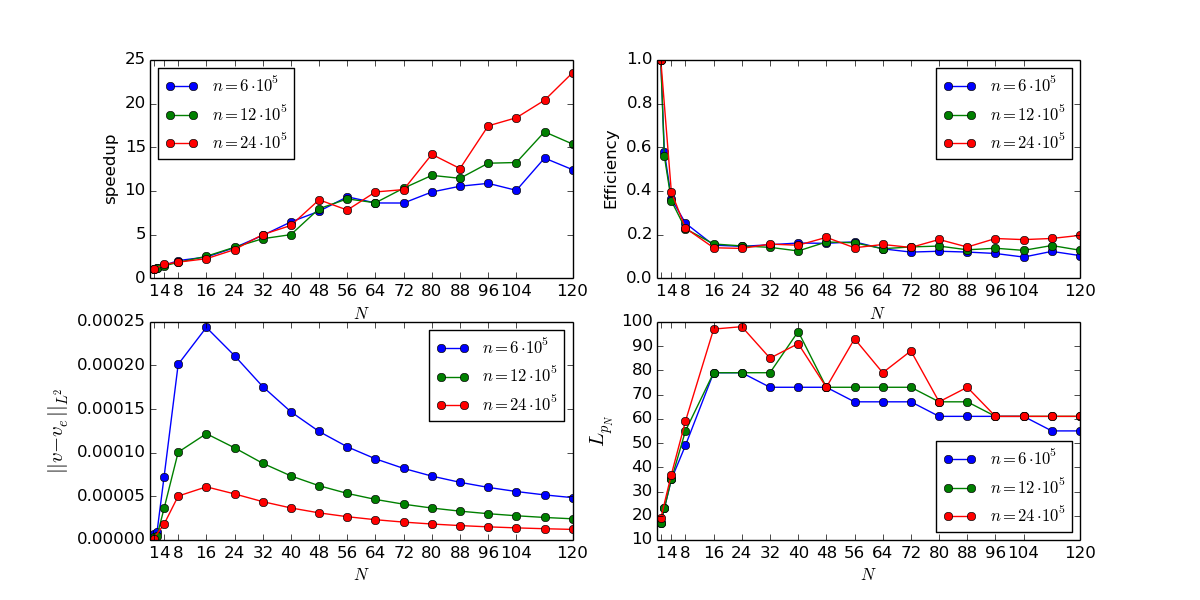
\includegraphics[scale=0.5]{fspeed_fig.png}
\centering
\caption{Speedup, efficiency, total number of objective function and gradient evaluations  ($L_{p_N}$) and relative norm error for problem (\ref{speed_j}-\ref{speed_e}) solved using $n=6\cdot 10^5,12\cdot 10^5,24\cdot 10^5$ time steps on $N$ cores.}
\label{speed_fig1}
\end{figure}
\\
\\
By looking at figure \ref{speed_fig1}, we see that our algorithm preformed the best, at least in the sense of speedup, for $n=24\cdot 10^5$. We do however also observe the same type of behaviour for all values of $n$. We see that the error between exact and numerical control solution for all $n$ first increases up till around $N=16$, and then decreases and flattens out. The total number of gradient and function evaluations $L_{p_N}$ becomes larger for higher $N$s when $N\leq 16$, but for $N>16$ $L_{p_N}$ starts to decrease slightly.  